%Chapter 4 gets to implementation. Explain each pipeline algorithm in sequence
\chapter{Implementation}
\label{chap:implementation}
This chapter will explore in great detail the functionality and implementation of this thesis's pipeline. As a reminder, the pipeline consists of the highlighted elements in Figure~\ref{fig:toplevelpipeline}. Each section of this chapter describes the implementation of one of these functional blocks.

\section{RGB-D Framework Library}
A crucial component of the pipeline is being able to easily collect RGB-D sensor data from a variety of sources in such a way that the origin of the data is hidden from the remainder of the pipeline. To that end, a highly modular and easily extensible event based framework library was built to seamlessly convert the native data formats and streaming behavior of different sensors. Figure~\ref{fig:rgbdframework} provides an overview of the framework organization. The application code deals directly with four primary classes: RGBDDevice, RGBDFrame, EventListeners, and FrameLogger.
\begin{figure}[ht]
    \centering
    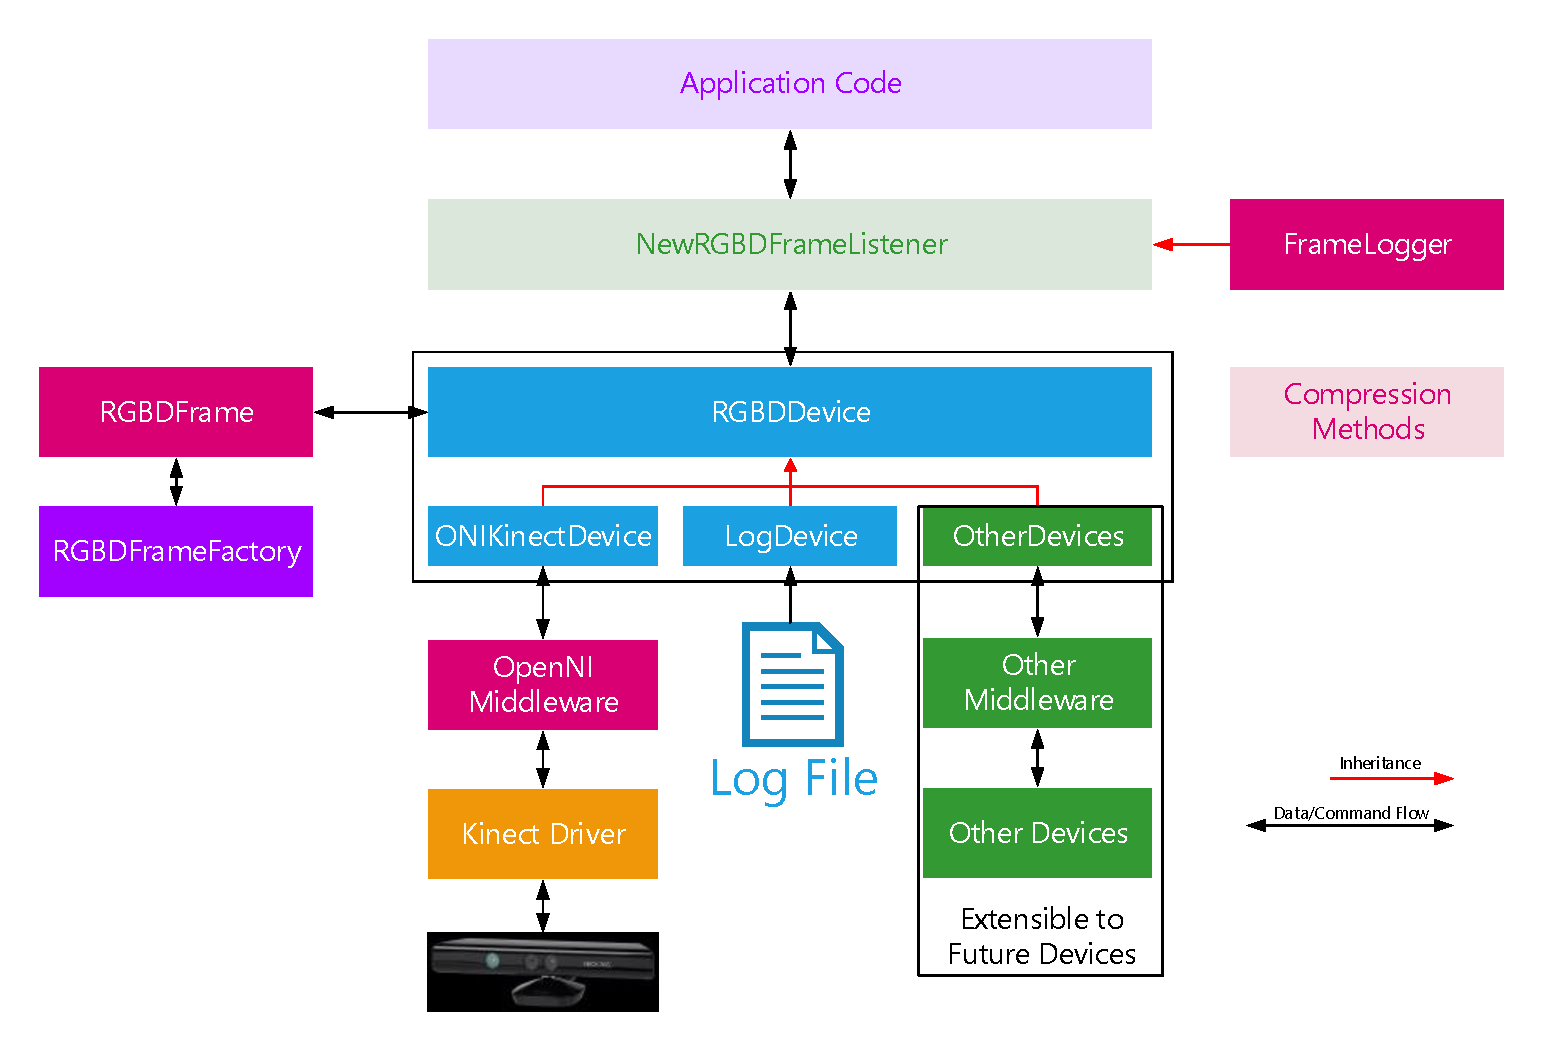
\includegraphics[width=1.0\textwidth]{FrameworkLayout.pdf}
    \caption{RGB-D framework architecture}
    \label{fig:rgbdframework}
\end{figure}
\subsection{RGBDDevice}
The primary interface between the framework and the rest of the application is the abstract class RGBDDevice. RGBDDevice provides an abstract interface including a data stream management API, access to device properties like camera intrinsics and resolution, and event listener registration API. Interfaces for specific devices like the Kinect can be implemented by creating a subclass of RGBDDevice and implementing the abstract methods. The application can then instantiate the desired subclass with device specific initialization parameters and the remainder of the pipeline can be completely agnostic to the underlying nature of the data source, since all RGBDDevices provide the same format RGBDFrame through the same event architecture regardless of the native device formatting. The current framework contains two subclasses: ONIKinectDevice and LogDevice. 
\paragraph{ONIKinectDevice} ONIKinectDevice implements a connection specific to the Microsoft Kinect using OpenNI as middleware. The implementation utilizes OpenNI's event-based interface to receive data from the sensor. Two streams for the color and depth data are created and registered with listeners internal to ONIKinectDevice. When a new depth or color frame is received from OpenNI, the data is copied and repackaged into an RGBDFrame format and a new thread is launched which passes the RGBDFrame to each registered listener. 
\paragraph{LogDevice} LogDevice replays a data log created using the FrameLogger class. Because of the way that the FrameLogger records the data, any device that can be implemented as an RGBDDevice can be recorded and played back using a LogDevice. The framework even allows logging data from a LogDevice. This class allows experiments to be performed very easily on prerecorded data without having to alter the behavior of the pipeline at all.
\subsection{RGBDFrame}

\subsection{NewRGBDFrameListener}

\subsection{FrameLogger}




\section{Filtering and Point Cloud Generation}
\section{Plane Segmentation}
\section{Planar Mesh Generation}